% Define document class
\documentclass[twocolumn]{aastex631}
%\documentclass[a4paper,aps,prl,amsfonts,amssymb,amsmath,nobibnotes,twocolumn,twoside,balancelastpage,eqsecnum] {revtex4-1}
\usepackage{showyourwork}
% \usepackage{datatool, filecontents}
% \DTLsetseparator{,}% Set the separator between the columns.
% \DTLloaddb[noheader, keys={thekey,thevalue}]{mydata}{output/ron_estimates.dat}
% Loads mydata.dat with column headers 'thekey' and 'thevalue'
% \newcommand{\var}[1]{\DTLfetch{my_data}{thekey}{#1}{thevalue}}
% Begin!
\begin{document}

% Title
\title{An open source scientific article}

% Author list
\author{{Freja Amalie Nørby (xvg720), Jacob Osman Hjortlund (nwl935) \& Martin Eriksen (bcm388)}}


% Abstract with filler text
\begin{abstract}
    balbalablabla balbalablabla balbalablabla balbalablabla balbalablabla balbalablabla balbalablabla balbalablabla balbalablabla balbalablabla
\end{abstract}

% Main body with filler text
\section{Introduction}
\label{sec:intro}

This report is a compilation of our progress in calibrating astronomical imaging data for the course Astronomical Data Processing. Our focus has been on mitigating various sources of noise and enhancing image quality through calibration of dark current, flat sky, lampflat, and bias images. Following a chronological order in alignment with the exercise sheets, we initiate with bias calibration and progress systematically through subsequent calibrations. The objective is to present a detailed account of our procedures and highlight the improvements achieved at each step, bla bla bla   bla bla bla 


\section{Image Calibration}
\label{sec:im_cal}

This section of the report will detail the steps for calibration, however we start with a introducing the observations we want to calibrate.

The observations or science files, we wish to calibrate, are of Messier 67 or NGC 2682, which is an open cluster located at a distance of roughly 2.7 kly. The observations were captured using the ESO Faint Object Spectrograph and Camera version 2 (EFOSC2), which at the time was mounted on the 3.6m telescope at the La Silla Observatory. The wavelength range of operation spans from 305nm to 1100nm, and the field of view measures 5.2'x5.2'. 

The observations consist of three data sets, all taken on December 30th, 2000, each with an exposure time of approximately 4.99 seconds. Accompanying these files were bias, dark and flat files taken at the same time. These files were filterd to only include file where the image had dimensions of 1030x1030 pixels, like the observations, which reduced the amount to 40 bias files, 6 dark files, 31 lampflat and 30 skyflat files. 

%https://www.eso.org/sci/facilities/lasilla/instruments/efosc/History.html
%https://www.ls.eso.org/sci/facilities/lasilla/instruments/efosc-3p6/Instrument_Overview.html

The calibration consists of three steps: 
\begin{enumerate}
    \item Analyse bias files and create a master bias file
    \item Analyse dark files and create a master dark file
    \item Analyse flat files and create a master flat file
\end{enumerate}

\subsection{Bias Correction}
\label{subsec:bias}
The bias files represent the offset in voltage applied to the CCD chip to ensure there are no negative counts during readout. 
Fig. \ref{fig:random_bias} Shows four random bias files form the filtered files. 
\begin{figure}[ht!]
\script{figures/random_bias_frames.py}
    \begin{centering}
        \includegraphics[width=\linewidth]{figures/random_bias_frames.pdf}
        \caption{Plot showing 4 random bias frames.}
        \label{fig:random_bias}
    \end{centering}
\end{figure}


\begin{figure}[ht!]
\script{figures/random_bias_frames.py}
    \begin{centering}
        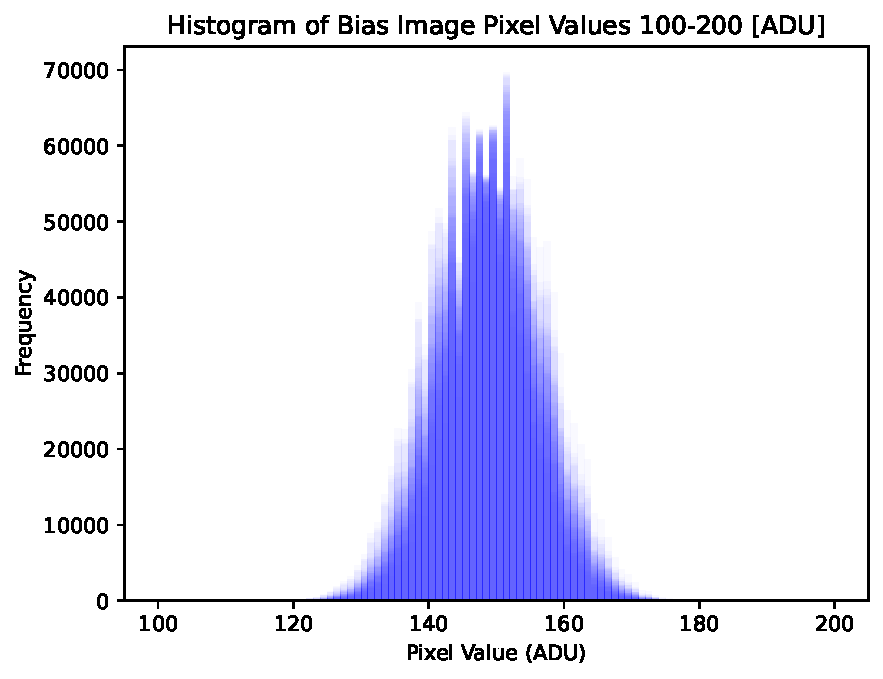
\includegraphics[width=\linewidth]{figures/biases_all_hist.pdf}
        \caption{}
        \label{fig:hist_all_bias}
    \end{centering}
\end{figure}

%inset picture of the STATS fig and the total histogram of the bias files

To find the pixels statistics of the bias files we divide the files into four quadrants, excluding a border of 20 pixels, and measure the mean, max, min and standard deviation of the quadrants as well as the entire FOV, again excluding the border of 20 pixels. As we can see in Fig. \ref{fig:bias_STATS} the minimum values of the four quadrants are very similar. The maximum value tends to either fall in the first or the third quadrant, and the mean shows that the first and second quadrants have the lowest mean value. When looking at the bias files there is a tendency towards slightly higher bias levels in the bottom half of the image along with some random dots here and there, but no strong features appear. When looking at the histogram of the bias values in Fig. \ref{fig:hist_all_bias} we also see that besides a few outliers the histogram is a nice Gaussian shape. 

\begin{figure}[ht!]
\script{figures/random_bias_frames.py}
    \begin{centering}
        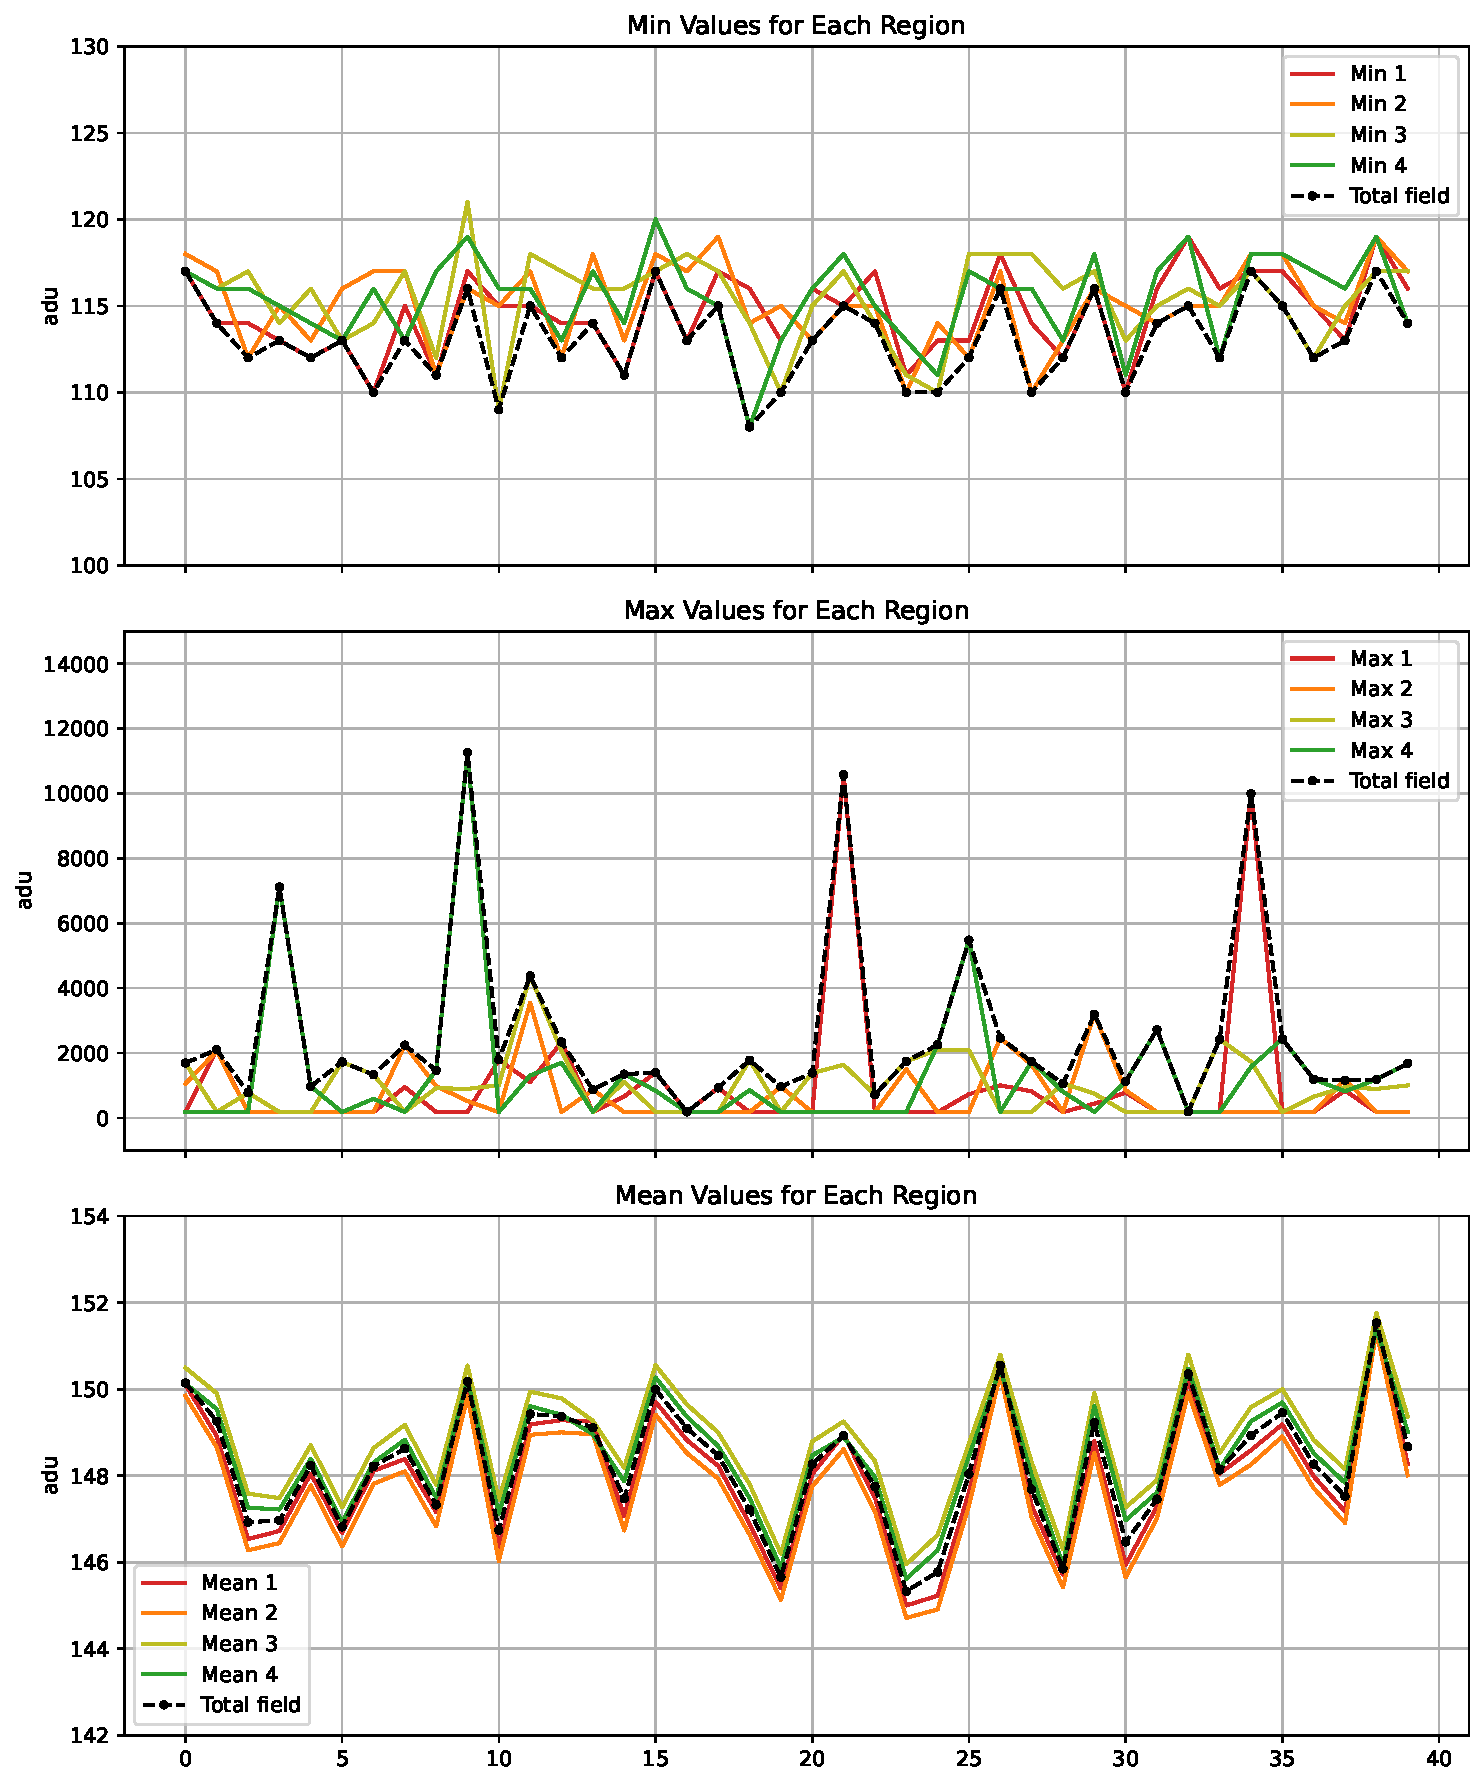
\includegraphics[width=\linewidth]{figures/bias_all_STATS_images.pdf}
        \caption{}
        \label{fig:bias_STATS}
    \end{centering}
\end{figure}

The master bias frame is created by combining all 40 bias frames using an average combining and applying a $\sigma$-clipping with a $\pm3\sigma$-thresholds. The resulting master bias file can be seen at Fig. \ref{fig:master_bias}.

\begin{figure}[ht!]
    \script{figures/master_bias_frame.py}
    \begin{centering}
        \includegraphics[width=\linewidth]{figures/master_bias_frame.pdf}
        \caption{
            Master Bias frame created using 40 frames. Outliers excluded using $\sigma$-clipping with median and MAD-STD with $\pm3\sigma$-thresholds. Frames combined using averaging.
        }
        \label{fig:master_bias}
    \end{centering}
\end{figure}


\begin{figure}[ht!]
    \script{figures/master_bias_stds.py}
    \begin{centering}
        \includegraphics[width=\linewidth]{figures/master_bias_stds.pdf}
        \caption{The left subplot  displays the mean signal as a function of the number of bias frames used to create the master frame. As the number of bias frames increases, the mean signal stabilizes. 
        The right subplot illustrates the standard deviation of the signal as function of the number of bias frames used to create the master frame. As the number of bias frames used in master frame creation increases, the standard deviation decreases.}
        \label{fig:bias_frame_stats}
    \end{centering}
\end{figure}
We were also tasked with creating a secondary master bias file using a limited number of bias files and analyzing the differences. In Fig. \ref{fig:bias_frame_stats}, we demonstrate how both the mean signal and the standard deviation in the combined images are minimized as we combine an increasing number of bias frames. It clearly demonstrates that the optimal choice for the number of bias frames is to use the maximum number of frames available. The combining function of averaging ensures the elimination of random noise patterns that may appear as isolated dots in some files and not in others, affirming that this noise is random and not a structural bias inherent to the instrument.

\subsection{Dark Current Correction}
\label{subsec:darks}
Dark frames are long exposure measurements with a closed shutter to record the background level of dark current in the instrument. When doing any kind of long exposure shots, a series of dark frames should always be taken to improve the signal to noise ratio of the processed data. Using our previously produced master bias frame we subtracted the bias level from the dark frames and then combined the processed dark frames, as previously explained for bias frames, into a master dark frame seen in \ref{fig:master_dark}. We find the dark current of the detector to be [AAAAAAAAAAAAAAAAAAAAAAAAAA], which becomes equal to the RON at [AAAAAAAAAAAAAAAAAAAAAAAAA].
\begin{figure}[ht!]
    \script{figures/master_dark_frame.py}
    \begin{centering}
        \includegraphics[width=\linewidth]{figures/master_dark_frame.pdf}
        \caption{}
        \label{fig:master_dark}
    \end{centering}
\end{figure}

\subsection{Flat Fielding}
\label{subsec:flats}
Flat field frames are taken using an evenly illuminated surface and are used to calculate the relative pixel to pixel sensitivity of the CCD. After calibrating data with a master flat field the processed data will be flattened and have a uniform output. In our image calibration we're using both lampflats and skyflats to calibrate our scientific data. The skyflats are taken in 3 different filters; B, V, and R, while the lampflats are taken in the V and R filters. A common way of acquiring skyflats are by using the twilight sky as the evenly illuminated surface, this has the advantage of exactly representing the sky background including emission lines, and they have the disadvantage of only being available during twilight. Lamp flats are much more convenient in this regard as it just requires an evenly illuminated white background to observe. When computing the standard deviation of the flatfield images we get []. Before creating our master flat fields we first calibrate both the skyflats and lampflats with our master dark, and bias frames. A master flat field is then created for every filter of both the lampflats, and the skyflats as seen in \ref{fig:master_skyflat} and \ref{fig:master_lampflat}. Since a change in illumination or exposure time would throw off the flux levels between flat field images we normalize the data to avoid this. [How did we do this? Did the flatfields have any vignetting?]


\begin{figure}[ht!]
    \script{figures/master_skyflat_frames.py}
    \begin{centering}
        \includegraphics[width=\linewidth]{figures/master_skyflat_frames.pdf}
        \caption{}
        \label{fig:master_skyflat}
    \end{centering}
\end{figure}

\begin{figure}[ht!]
    \script{figures/master_lampflat_frames.py}
    \begin{centering}
        \includegraphics[width=\linewidth]{figures/master_lampflat_frames.pdf}
        \caption{}
        \label{fig:master_lampflat}
    \end{centering}
\end{figure}

\subsection{Science Image Calibration}
\label{subsec:im_cal}

%lest start by giving a short intro to our fits files, how many science files, and which clusere they are form, and which instrumnet were used to create the files

\begin{figure}[ht!]
    \script{figures/skyflat_calibrated_science_images.py}
    \begin{centering}
        \includegraphics[width=\linewidth]{figures/skyflat_calibrated_science_images.pdf}
        \caption{}
        \label{fig:master_dark}
    \end{centering}
\end{figure}

\begin{figure}[ht!]
    \script{figures/lampflat_calibrated_science_images.py}
    \begin{centering}
        \includegraphics[width=\linewidth]{figures/lampflat_calibrated_science_images.pdf}
        \caption{}
        \label{fig:master_dark}
    \end{centering}
\end{figure}

\begin{figure}[ht!]
    \script{figures/skyflat_calibrated_standard_star_images.py}
    \begin{centering}
        \includegraphics[width=\linewidth]{figures/skyflat_calibrated_standard_star_images.pdf}
        \caption{}
        \label{fig:master_dark}
    \end{centering}
\end{figure}

\begin{figure}[ht!]
    \script{figures/lampflat_calibrated_standard_star_images.py}
    \begin{centering}
        \includegraphics[width=\linewidth]{figures/lampflat_calibrated_standard_star_images.pdf}
        \caption{}
        \label{fig:master_dark}
    \end{centering}
\end{figure}


\bibliography{bib}

\end{document}
